%!TEX root = ../thesis.tex
% ******************************* Thesis Appendix B ********************************

\chapter{Further Image Comparisons}
\label{chapter:appendix_b}

\graphicspath{{../img/plots/kodak_comparison/}{../img/plots/kodak_coding_time/}{../img/plots/kodak_side_info/}{../img/plots/reconstructions/}}


\par In this appendix we present some further reconstruction comparisons for the
models we trained. All of the plots presented in this appendix as well as plots
for images are available online at
\url{https://github.com/gergely-flamich/miracle-compression/tree/master/img/plots}. 

\paragraph{}
The images and their statistics are displayed in the following order:
\texttt{kodim04}, \texttt{kodim10} and \texttt{kodim17}.
For each image, we first present their regular PLN and then their $\gamma$-PLN
reconstructions.
The $\beta$s corresponding to the images in the quartered comparison plots are
shown in Table \ref{tab:beta_layout}.
We also present the compression comparison plot and the side information plot
as described in Chapter \ref{chapter:experiments}.
\begin{table}[H]
  \centering
  \begin{tabular}{|r|c|c|c|c|}
    \hline
    & \textbf{Top Left} & \textbf{Top Right} & \textbf{Bottom Left} & \textbf{Bottom Right} \\
    \hline\hline
    Regular PLNs & 0.03 & 0.1 & 0.3 & 1 \\
    \hline
    $\gamma$-PLNs & 0.1 & 1 & 3 & 10 \\
    \hline
  \end{tabular}
  \caption{$\beta$s used in the quartered comparison plots for PLNs and $\gamma$-PLNs.}
  \label{tab:beta_layout}
\end{table}


% ======================================================================
% Kodak 04
% ======================================================================
\begin{figure}
  \centering
  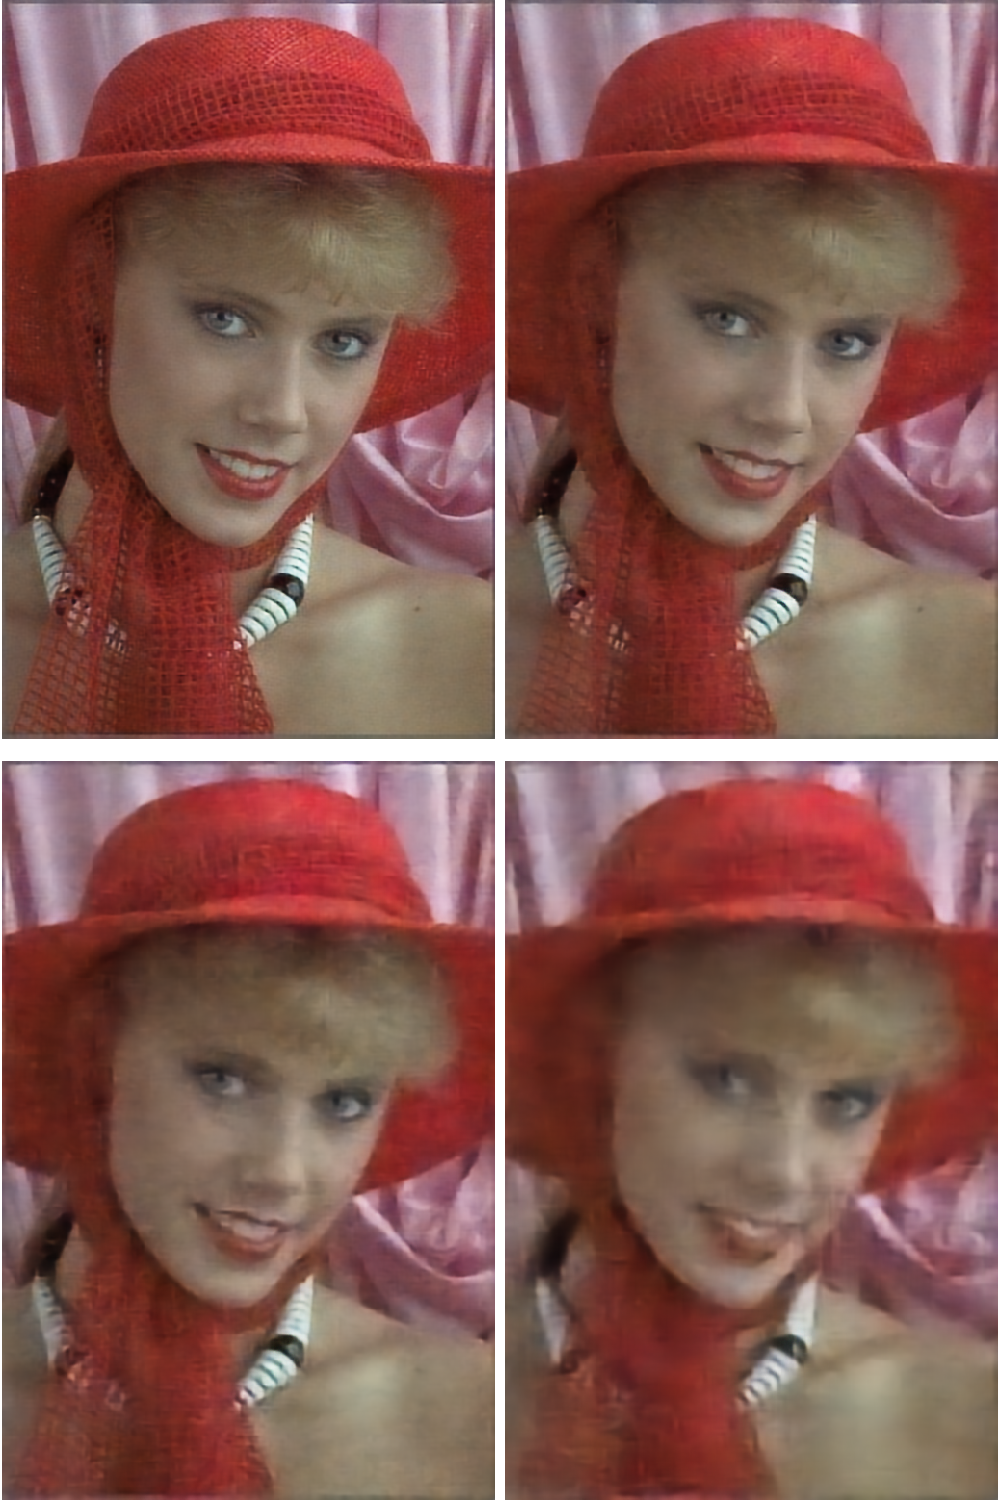
\includegraphics[width=\textwidth]{pln_003_01_03_1_k04.png}
\end{figure}
\begin{figure}
  \centering
  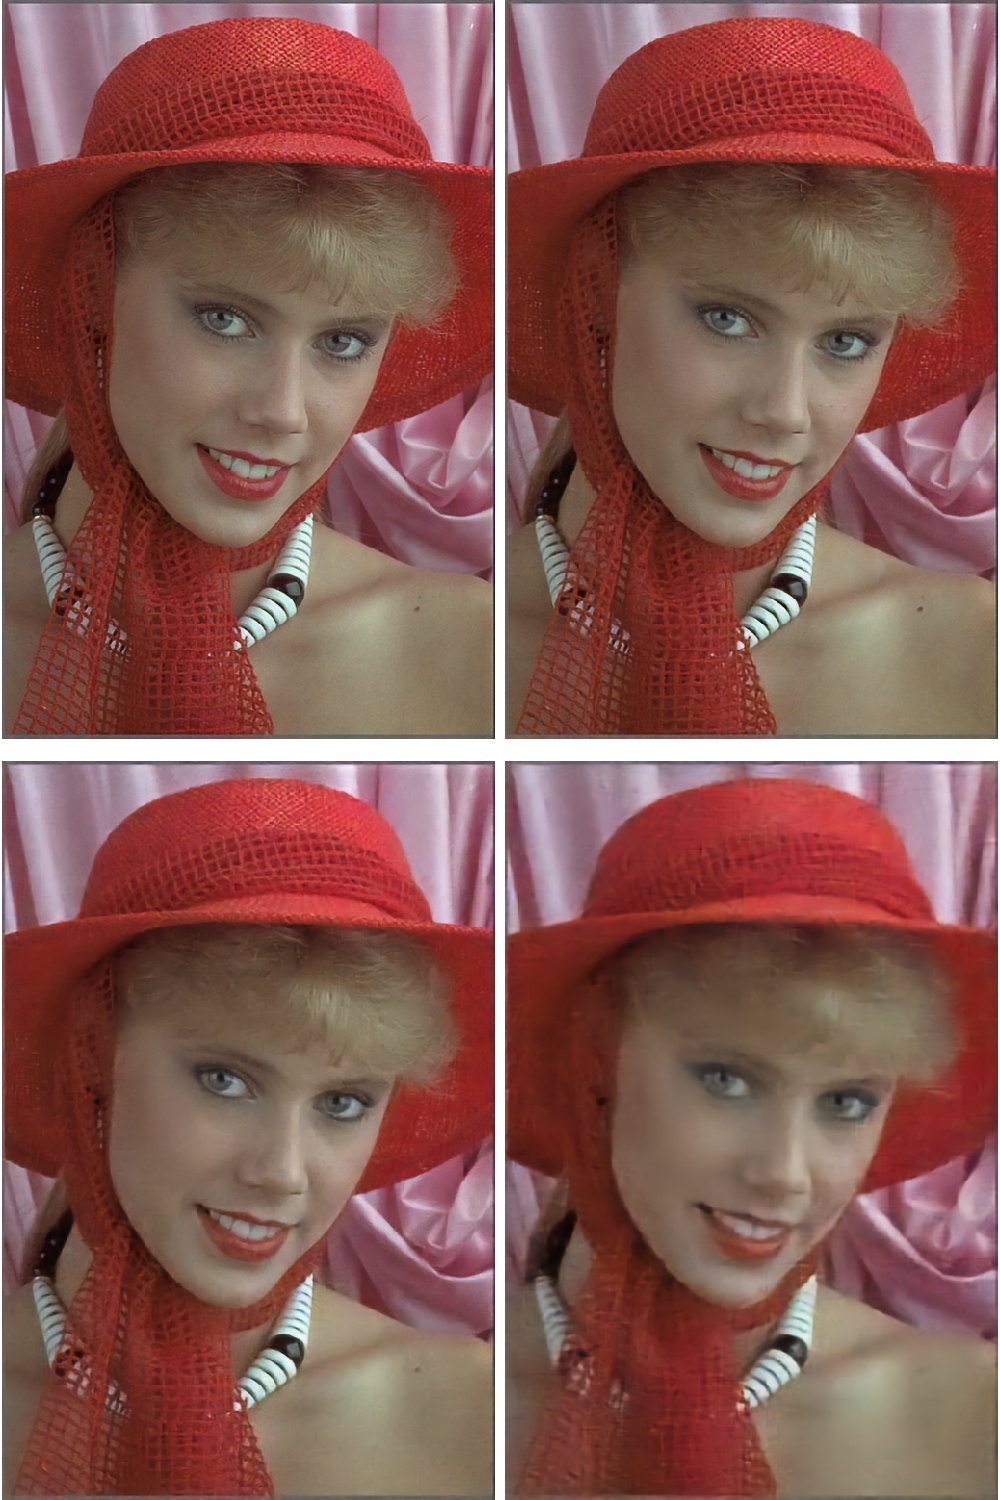
\includegraphics[width=\textwidth]{log_gamma_01_1_3_10_k04.png}
\end{figure}
\begin{figure}
  \centering
  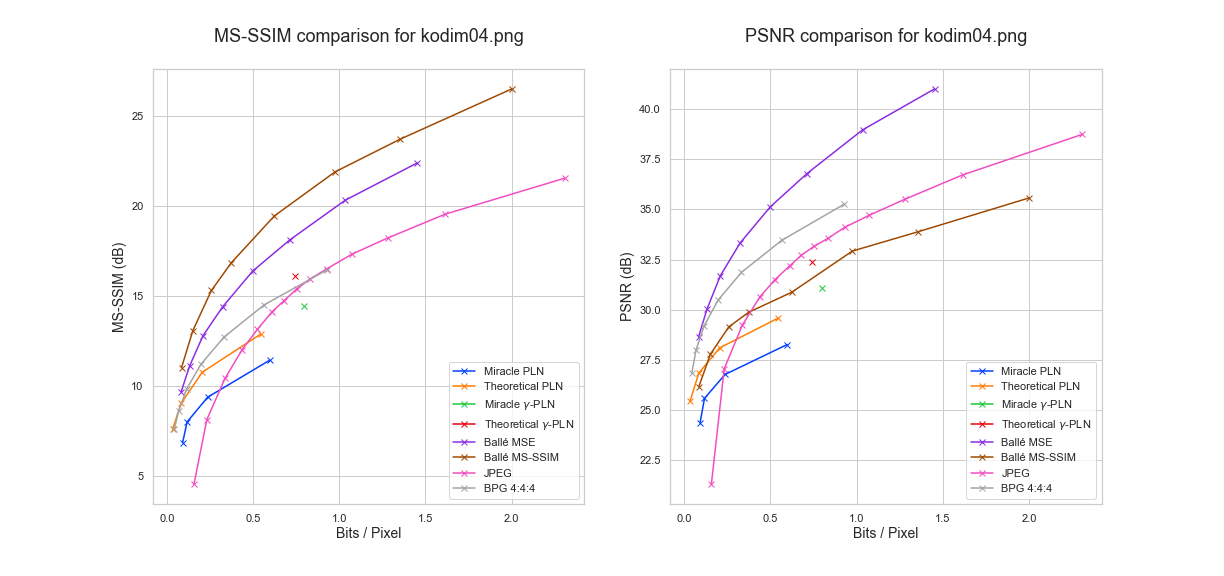
\includegraphics[width=\textwidth]{kodim04_comparison.png}
\end{figure}
\begin{figure}
  \centering
  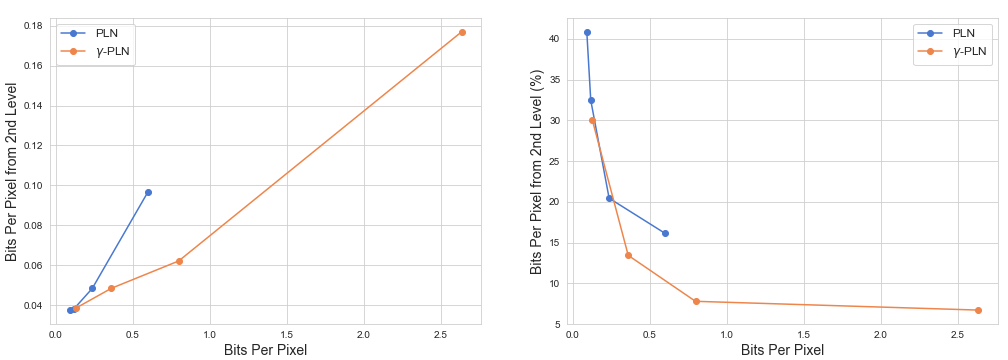
\includegraphics[width=\textwidth]{kodim04_side_info.png}
\end{figure}

% ======================================================================
% Kodak 10
% ======================================================================
\begin{figure}
  \centering
  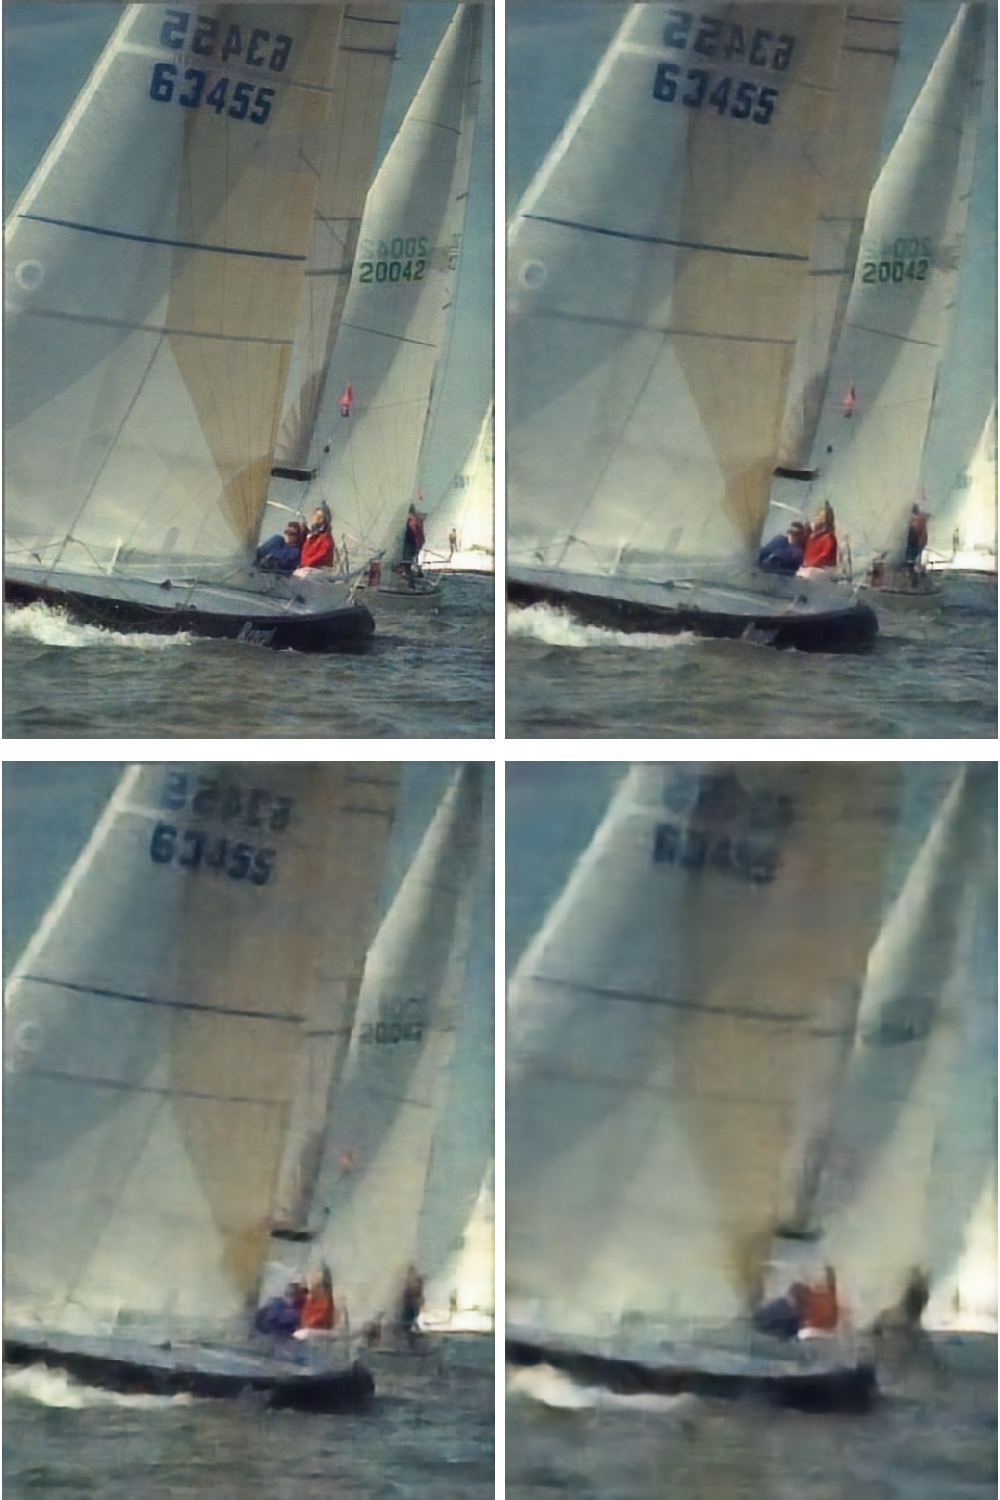
\includegraphics[width=\textwidth]{pln_003_01_03_1_k10.png}
\end{figure}
\begin{figure}
  \centering
  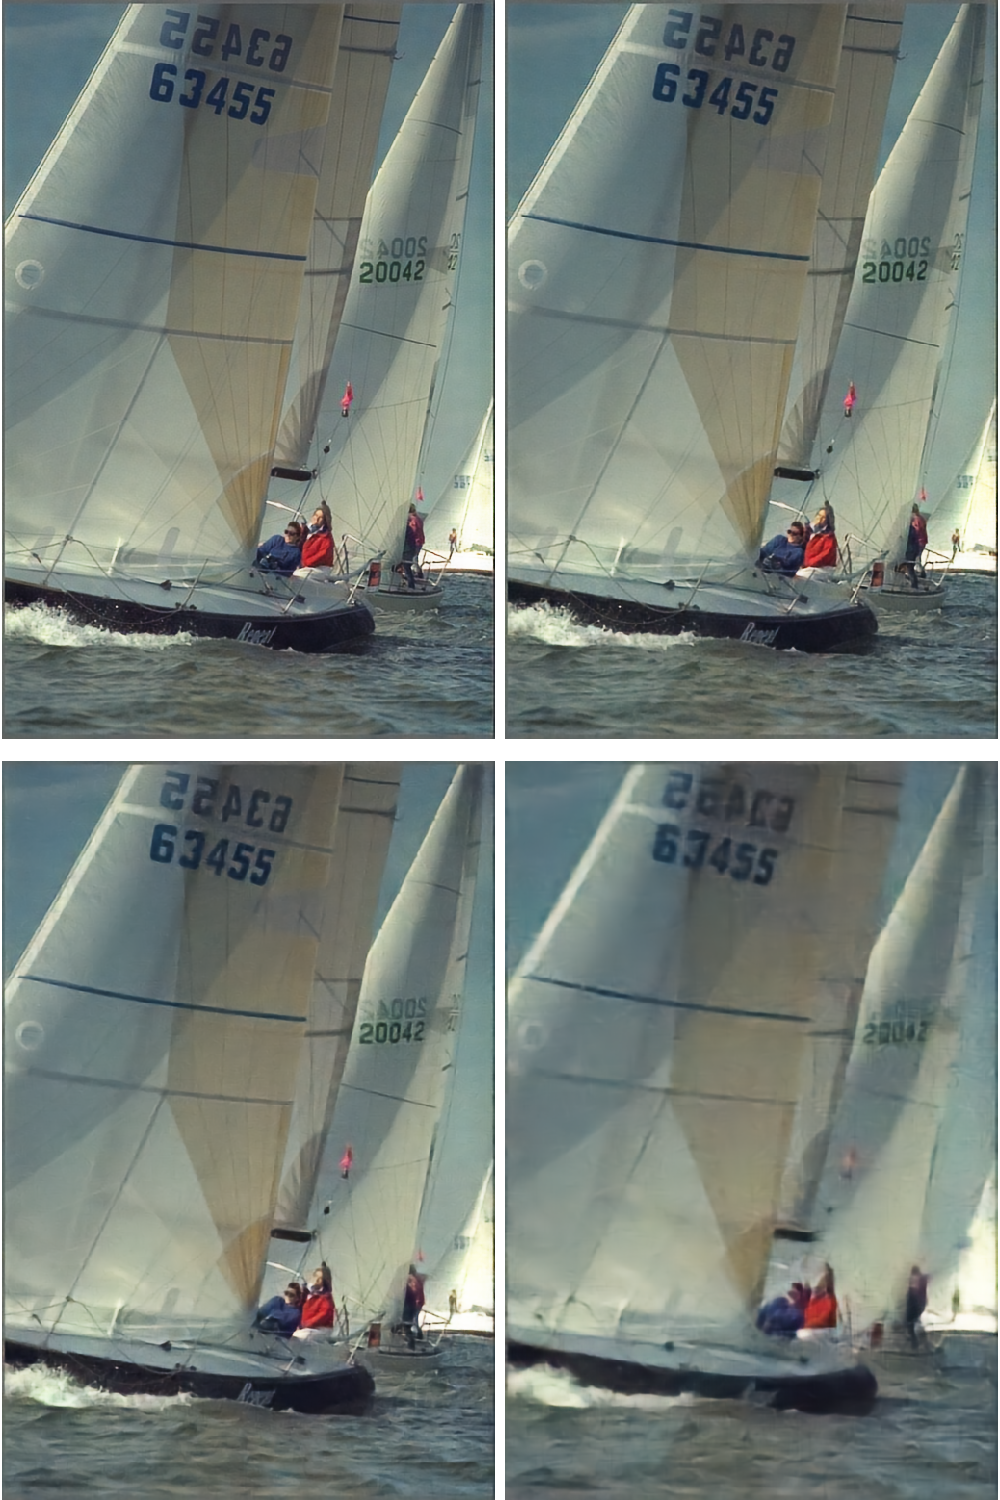
\includegraphics[width=\textwidth]{log_gamma_01_1_3_10_k10.png}
\end{figure}
\begin{figure}
  \centering
  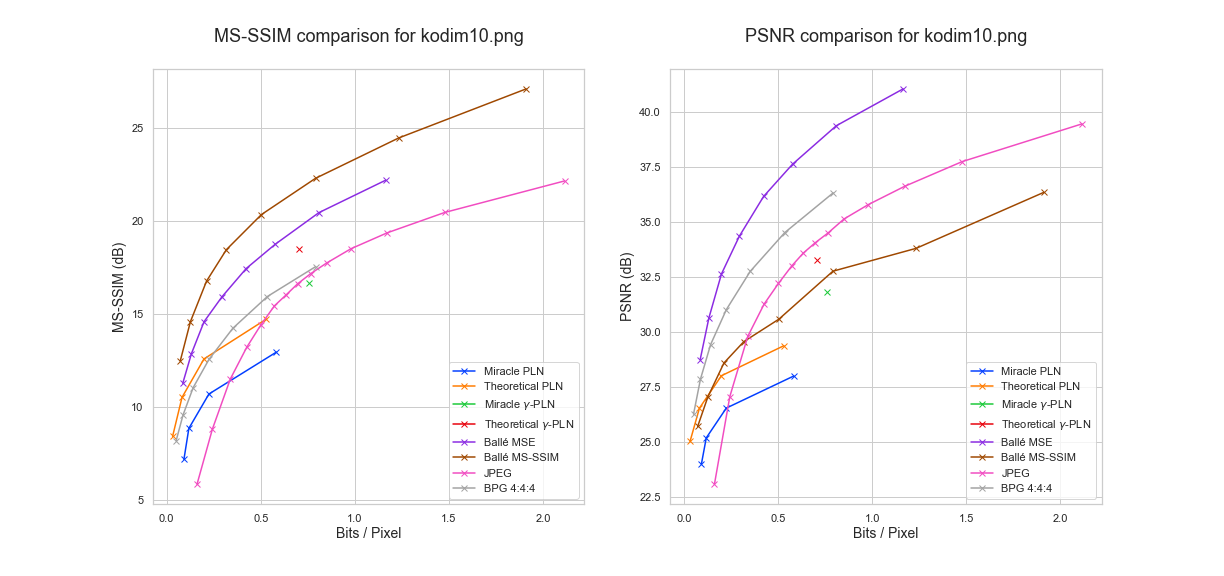
\includegraphics[width=\textwidth]{kodim10_comparison.png}
\end{figure}
\begin{figure}
  \centering
  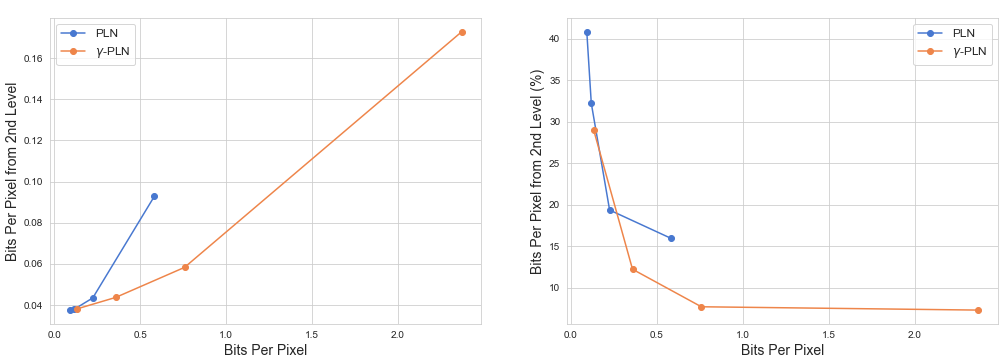
\includegraphics[width=\textwidth]{kodim10_side_info.png}
\end{figure}

% ======================================================================
% Kodak 17
% ======================================================================
\begin{figure}
  \centering
  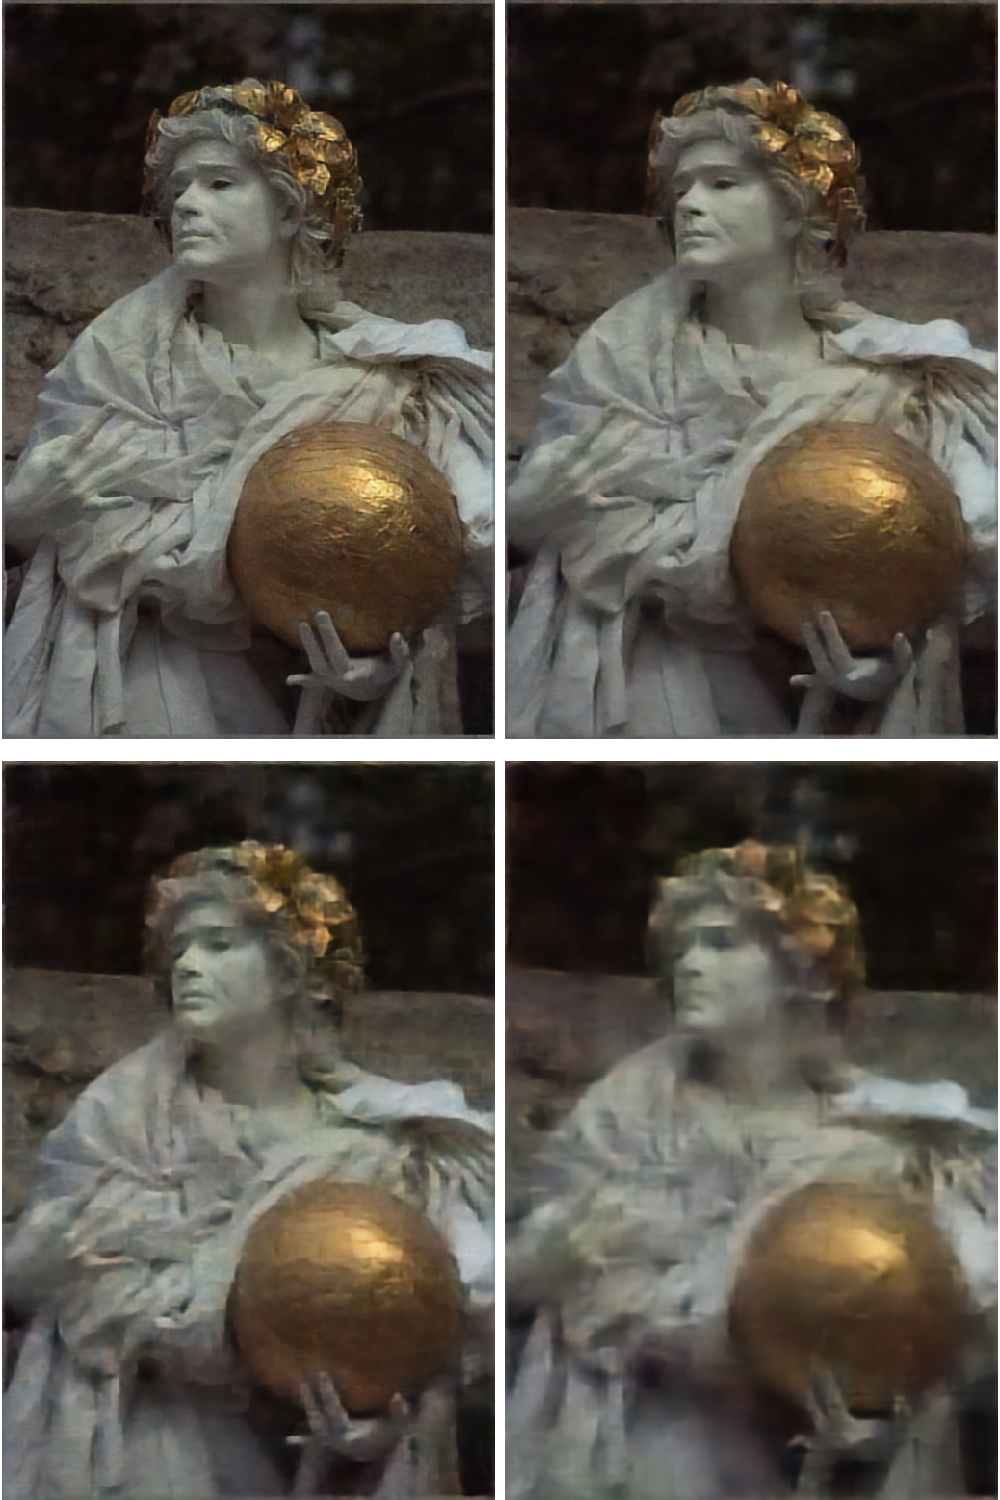
\includegraphics[width=\textwidth]{pln_003_01_03_1_k17.png}
\end{figure}
\begin{figure}
  \centering
  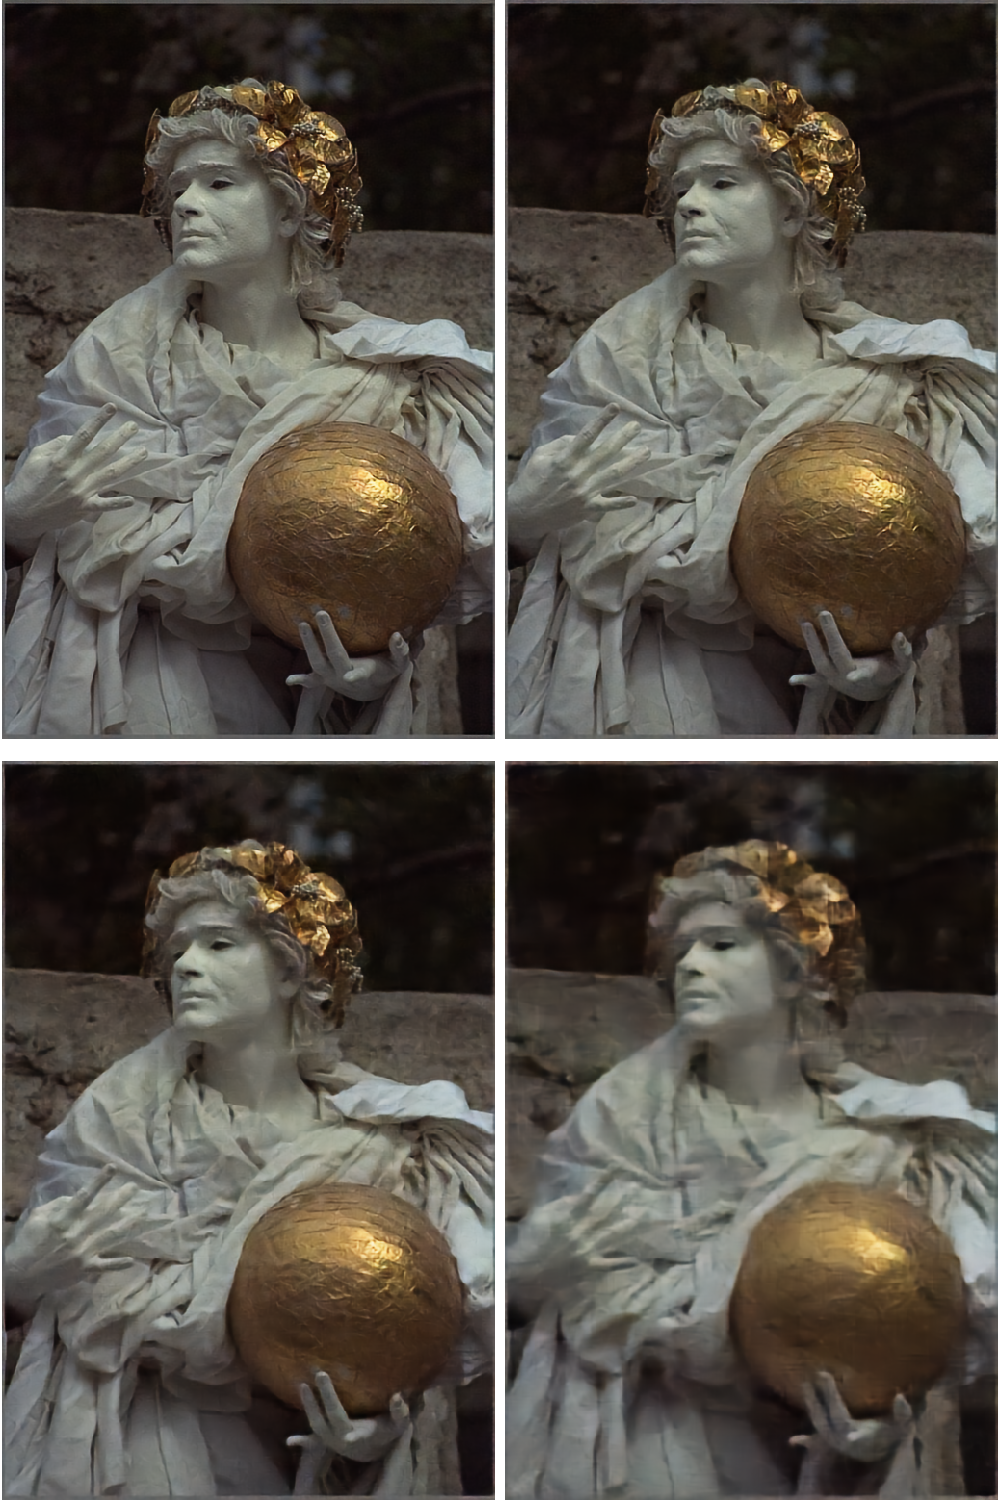
\includegraphics[width=\textwidth]{log_gamma_01_1_3_10_k17.png}
\end{figure}
\begin{figure}
  \centering
  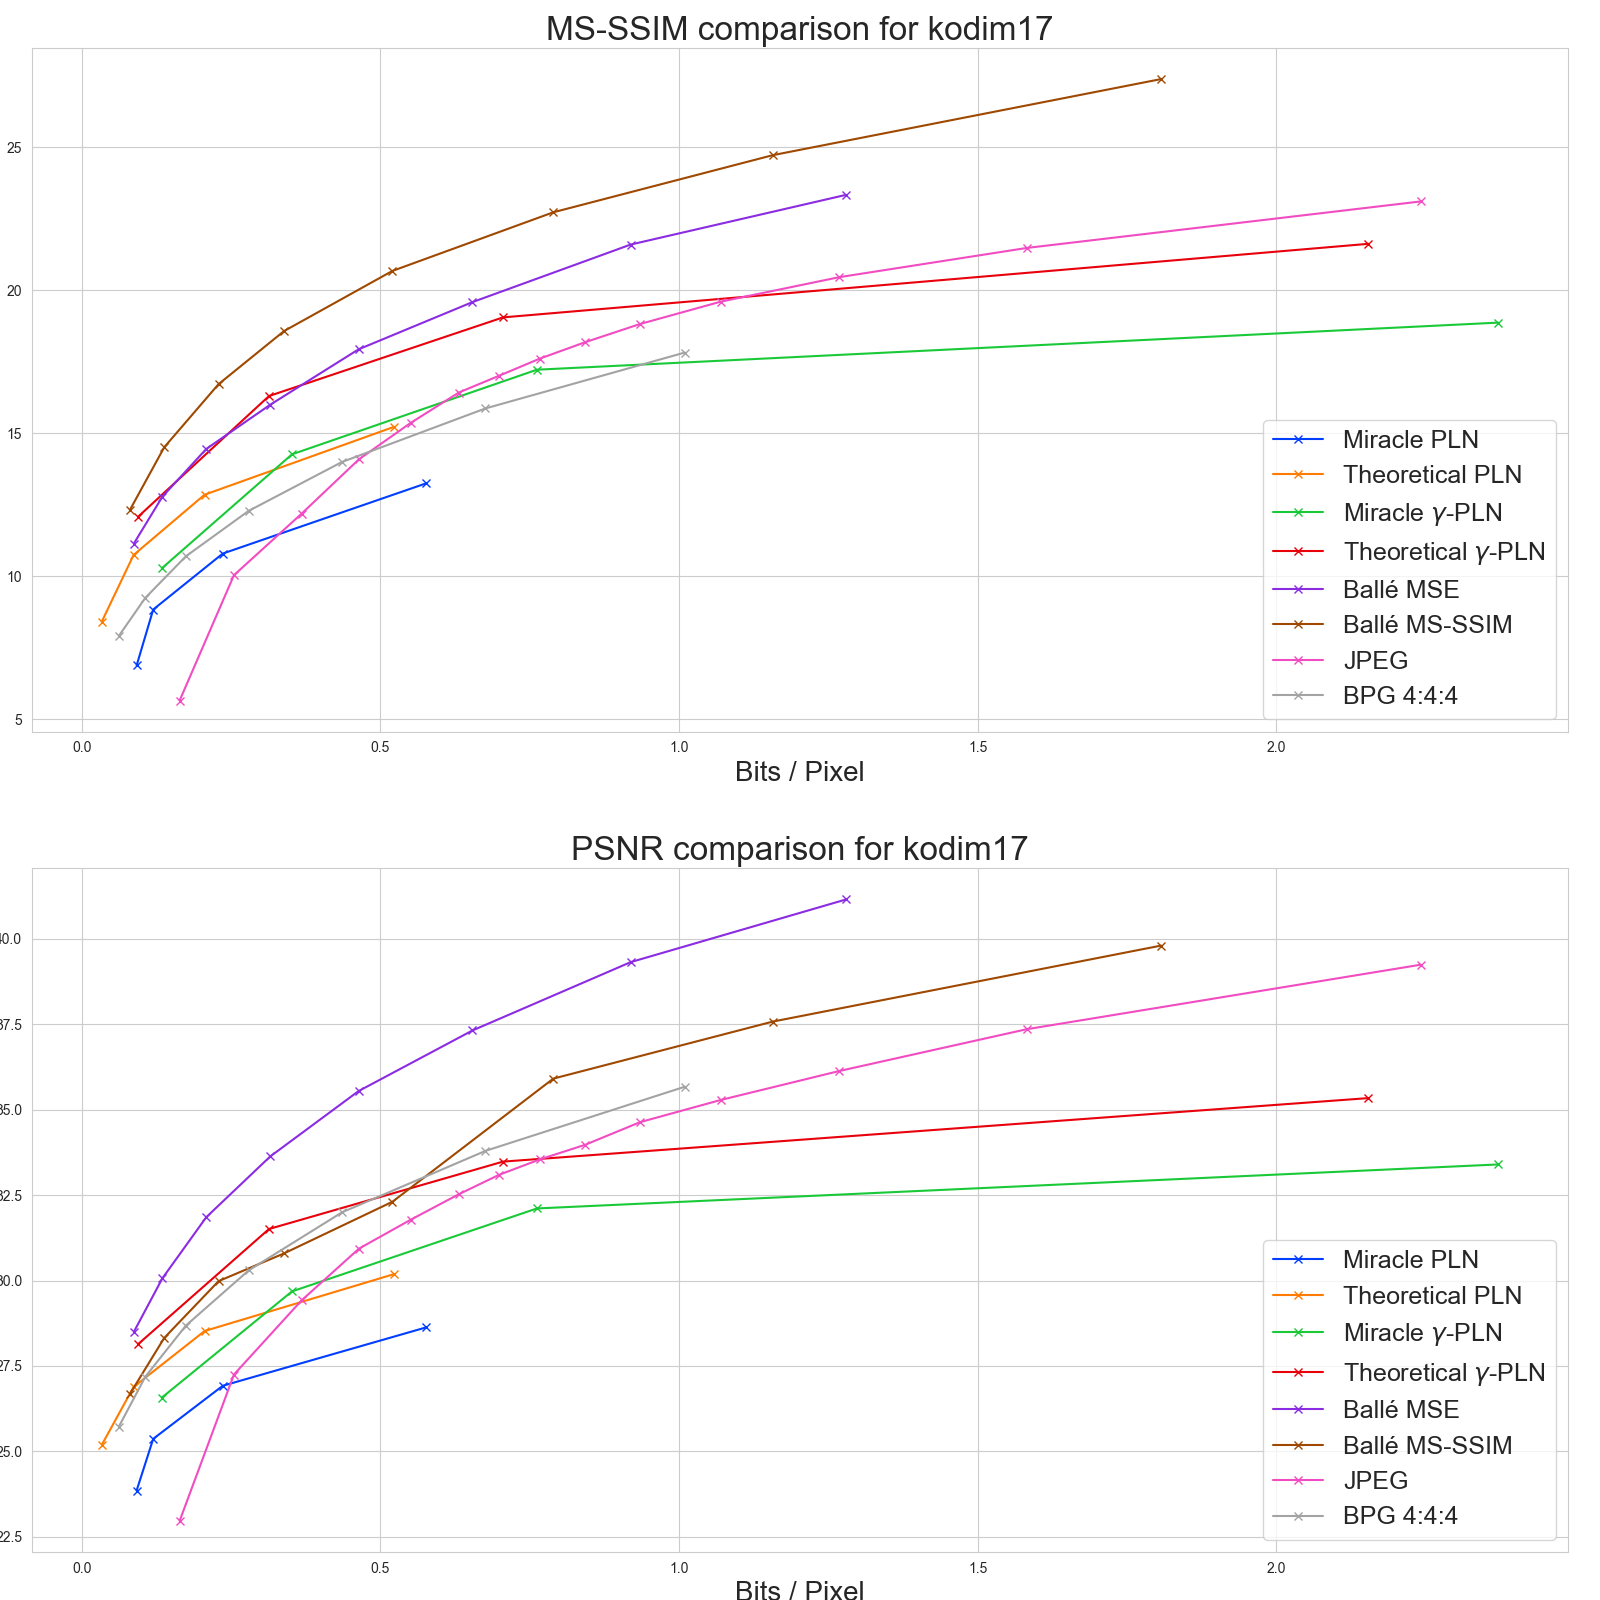
\includegraphics[width=\textwidth]{kodim17_comparison.png}
\end{figure}
\begin{figure}
  \centering
  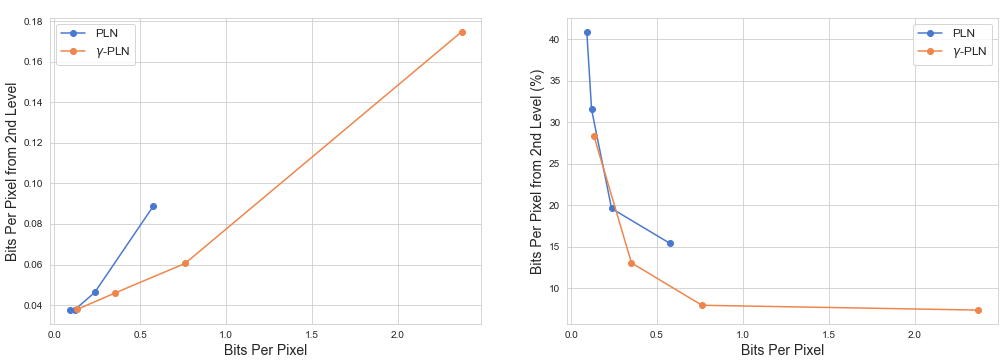
\includegraphics[width=\textwidth]{kodim17_side_info.png}
\end{figure}